\documentclass[11pt,a4paper]{article}
\usepackage[T1]{fontenc}
\usepackage[utf8]{inputenc}
\usepackage{lmodern}
\usepackage[margin=24mm]{geometry}
\usepackage{microtype}
\usepackage{amsmath,amssymb}
\usepackage{booktabs,tabularx,array}
\usepackage{enumitem}
\usepackage[numbers,sort&compress]{natbib}
\usepackage{xcolor}
\usepackage{fancyhdr}
\usepackage{tikz}
\usetikzlibrary{positioning,arrows.meta}
\usepackage[colorlinks=true,linkcolor=blue!45!black,citecolor=blue!45!black,urlcolor=blue!45!black,breaklinks=true]{hyperref}
\setlength{\emergencystretch}{2em}
\setlength{\headheight}{14pt}
\setlist{nosep,leftmargin=*}
\newcolumntype{Y}{>{\raggedright\arraybackslash}X}
\newcommand{\pending}[1]{\textcolor{blue!55!black}{\textbf{Pending evidence:} #1}}
\newcommand{\status}[1]{\par\smallskip\noindent\fcolorbox{black!20}{black!3}{\parbox{0.95\linewidth}{\small #1}}\par\smallskip}
\pagestyle{fancy}
\fancyhf{}
\fancyhead[L]{\small Research draft v0.1}
\fancyhead[R]{\small Empirical validation pending}
\fancyfoot[C]{\thepage}
\title{Diagnostic Skill Reuse for Agentic Autotuning\\of Disaggregated LLM Serving in SGLang}
\author{Author list to be supplied\\Tencent affiliation details to be confirmed}
\date{18 October 2026}

\begin{document}
\maketitle
\status{Design-stage manuscript. The literature review and proposed method are drafted; the integrated system has not been verified and performance experiments have not been conducted for this manuscript. Statements about the proposed system describe a design, not an implemented result. No numerical improvement, deployment outcome, or novelty-priority claim is asserted.}

\begin{abstract}
Configuring prefill--decode disaggregated large language model serving requires decisions about phase allocation, parallelism, request batching, and state transfer. A useful configuration must satisfy user-visible latency objectives while accounting for resource consumption and the cost of finding that configuration. We propose an agentic autotuning design in which a diagnostic skill is an executable experiment with explicit applicability conditions, alternative expected observations, and a record of supporting and contradicting evidence. A language-model controller selects diagnostic actions and parameter families; a constrained numerical optimizer proposes concrete configurations. Before reusing a skill in a changed workload or deployment, the controller checks compatibility and, when necessary, requests a local diagnostic replay. Skill guidance biases search without permanently excluding otherwise valid configurations. The intended distinction is the explicit decision to acquire and revalidate evidence about coupled serving stages, rather than the presence of an agent or a memory store. We formulate resource planning and tuning-cost objectives, specify a capability-aware SGLang integration, and define an evaluation that separates the effects of numerical search, agent decisions, and skill reuse. Validation on a P800 accelerator pool is planned. This draft reports no empirical results.
\end{abstract}

\noindent\textbf{Keywords:} LLM serving; prefill--decode disaggregation; agentic autotuning; diagnostic skills; resource planning.

\section{Introduction}
LLM serving systems expose configuration choices across resource allocation, parallel execution, memory management, batching, and communication. Prefill--decode (PD) disaggregation makes phase-specific choices possible, but also introduces explicit transfer of request state. DistServe studies phase allocation under latency constraints, Splitwise examines phase-specific hardware provisioning, and HexGen-2 jointly considers heterogeneous resources and communication~\cite{distserve2024,splitwise2024,hexgen2025}. These results establish that the stages and their connections should be considered together. They do not make PD deployment itself a new contribution of the present work.

This manuscript focuses on a decision that occurs before choosing a new configuration: \emph{which observation or controlled experiment should be obtained next?} Consider a deployment whose service objective is no longer met after the request mix changes. Adding a prefill instance, reducing decode admission, and changing an available transfer setting affect different parts of the execution. The same aggregate latency symptom may be consistent with several explanations. A tuner can search all choices numerically, but may spend substantial time redeploying configurations that do not address the current limitation. An agent can interpret heterogeneous evidence, but a plausible explanation alone does not validate a diagnosis.

The use of LLMs for tuning is established. GPTuner combines domain knowledge and numerical optimization, while STELLAR analyzes logs and accumulates contextual tuning rules. SysInsight links system internals, diagnosis, and empirically supported rules~\cite{gptuner2024,stellar2025,sysinsight2026}. Accordingly, adding tool calls, contextual memory, or rule confidence is not sufficient novelty. Our narrower research question is whether an explicit \emph{diagnostic experiment and its local replay conditions} provide useful decision structure for PD serving, where a deployment change can alter several connected stages.

We propose to represent a diagnostic skill as a bounded program that acquires observations capable of supporting, contradicting, or leaving unresolved a set of stage-related hypotheses. A controller can use the resulting evidence to prioritize a parameter family. The skill also records where its evidence was obtained. Reuse in a changed context requires compatibility checks and may require a new probe. This design treats a diagnosis as a revisable empirical statement, not as an instruction to repeatedly apply the last successful parameter adjustment.

The intended system has one LLM controller, a small engineering-authored diagnostic library, a numerical optimizer, and an independent executor and evaluator. Resource counts are variable. The initial target environment reported by the author is four eight-P800 servers with dual-socket AMD EPYC hosts and RDMA connectivity; a larger resource pool can be used as needed. These are available experimental conditions, not evidence that the proposed method is effective. AMD refers to host CPUs, not an additional accelerator backend.

This draft develops three research artifacts: a formulation of evidence acquisition and configuration selection under a shared tuning budget; a proposed diagnostic-skill representation with local reuse checks and nonexclusive search guidance; and an evaluation protocol that can test the necessity of both the agent and the skill mechanism. The first two are candidate method contributions. The third is the evidence required to assess them. Their empirical value and distinction from prior systems remain to be established.

\section{Background and Related Work}
\subsection{Disaggregated serving and configuration}
PD serving separates the processing of prompts and the generation of subsequent tokens across model replicas. The practical configuration space includes the number of replicas, their parallel strategies, runtime limits, and supported transfer paths. Mooncake organizes service around KV state, and Sarathi-Serve provides an important colocated alternative based on chunked prefill~\cite{mooncake2024,sarathi2024}. A fair evaluation must therefore consider a tuned colocated system as well as tuned native PD.

SGLang provides a language-model execution system and runtime~\cite{sglang2024}. Its current PD documentation and the SGLang-Kunlun repository provide relevant integration surfaces~\cite{sglangpd,kunlunplugin}. These evolving sources do not establish that every documented feature is available in the deployed P800 image. Our design requires a version-specific capability manifest and does not assume support for unequal tensor parallelism, a particular direct-memory path, or arbitrary replica routing.

Recent preprints also address SLO-aware PD resource counts and coordinated phase/network autoscaling~\cite{pdresources2026,tokenscale2025}. Variable resource counts and network-aware provisioning are therefore not gaps claimed here. Our initial planner recommends a deployment offline; it does not claim the online control mechanisms of an autoscaler.

\subsection{Numerical and knowledge-guided autotuning}
SCOOT applies constrained Bayesian optimization to inference-engine tuning and handles known and hidden configuration constraints~\cite{scoot2025}. It is a direct algorithmic reference for numerical search. GPTuner extracts tuning knowledge and uses it for knob selection and search-space optimization; $\lambda$-Tune generates complete database configurations and accounts for candidate-evaluation overhead~\cite{gptuner2024,lambdatune2025}. These works motivate comparisons against capable search and knowledge-guided methods rather than against defaults alone.

SLO-Guard studies failure-aware, budget-consistent serving tuning, while ECO combines a structured prior and constrained optimization for disaggregated serving under limited measurements~\cite{sloguard2026,ecotuning2026}. Both are preprints in the cited versions. Failure accounting, model-assisted search, and a limited tuning budget are consequently not standalone novelty claims of our design.

\subsection{Agents, diagnosis, and accumulated knowledge}
STELLAR already supports adaptive analysis, configuration execution, and accumulated rules with tuning contexts. Its rule synthesis also addresses conflicting guidance~\cite{stellar2025}. SysInsight derives hypotheses from code, induces contextual rules from observations, and maintains feedback-based reliability~\cite{sysinsight2026}. StorageXTuner, a preprint, combines agent roles, exploration, and empirically validated insights~\cite{storagextuner2025}. These mechanisms overlap substantially with a generic proposal for an agent with skills. We do not describe any of them as lacking context, feedback, or validation.

Our proposed distinction is an explicit action representation for \emph{diagnostic interventions}: what can be changed or observed, which competing stage explanations it can distinguish, and what evidence is required before transferring its guidance. Whether this representation provides more than an application-specific reimplementation is an empirical question. A matched agent baseline and a matched rule-based controller are essential.

\subsection{Measurement and comparison}
Autotuning comparison must account for elapsed time, stochasticity, and evaluation overhead~\cite{methodology2024}. AutoTuneBench, a recent preprint, studies the reliability of agent-generated serving and kernel measurements~\cite{autotunebench2026}. We adopt independent metric computation and complete accounting as experimental requirements; these safeguards are not claimed as the primary novelty of this manuscript.

\section{Problem Formulation}
\subsection{Tasks, configurations, and capabilities}
A task is $\tau=(m,w,h,v,\mathcal{S})$, where $m$ identifies the model and fixed precision policy, $w$ describes the externally supplied request process, $h$ describes the resource topology, $v$ identifies the software stack, and $\mathcal{S}$ specifies service objectives. Workload features include input and actual output length distributions, arrival variability, and cache-reuse conditions. A maximum output length is not a substitute for the measured distribution.

A configuration is
\begin{equation}
 c=(n_P,n_D,p_P,p_D,\pi,b_P,b_D,k),
\end{equation}
where $n_P,n_D$ are replica counts, $p_P,p_D$ are supported parallel strategies, $\pi$ maps workers to resources, $b_P,b_D$ are runtime limits, and $k$ contains supported state-transfer settings. The legal set $\mathcal{C}_{\tau}$ follows from the capability manifest, memory feasibility, and resource availability. Model and KV precision remain fixed within a comparison. Counts denote complete replicas, not arbitrary divisions of model weights.

Let $A(c)$ be the number of allocated accelerator cards; whole-node allocation is recorded separately when it determines reclaimable resources. We do not assume equal resource use per replica or that a model fits on a particular number of P800 cards. Structural changes can require redeployment. The first implementation is an offline planner; online elasticity and in-flight migration are outside its initial scope.

\subsection{Service feasibility and objectives}
For request $i$, define
\begin{equation}
 z_i(c)=\mathbf{1}\{\text{complete}_i \land f_i\leq\theta_f
                  \land o_i\leq\theta_o\},
\end{equation}
where $f_i$ is client-observed TTFT and $o_i$ is the request-level mean interval between output tokens. The primary workload will have at least two output tokens. Any shorter completions will be reported separately using a prespecified eligibility policy. Failures, timeouts, and rejected requests remain in the offered-request denominator.

For a fixed arrival cohort of $N$ requests,
\begin{equation}
 \widehat a(c)=\frac{1}{N}\sum_{i=1}^{N}z_i(c).
\end{equation}
For a stable offered arrival rate $\lambda$, $\lambda\widehat a(c)$ is an attained-arrival-rate estimate. We will distinguish it from completion-window throughput and will report the arrival, observation, and drain intervals. Queue stability and a fixed timeout policy are required to prevent short measurement windows from concealing overload. Separate marginal tail objectives do not imply the same joint attainment.

The capacity-planning objective is
\begin{equation}
 \min_{c\in\mathcal{C}_{\tau}} A(c)
 \quad\text{subject to}\quad
 a(c)\geq\alpha,\quad\text{stable queues}.
 \label{eq:capacity}
\end{equation}
The system will return the smallest \emph{measured feasible} configuration it has found, not a certified global optimum. Within an equal-resource stratum, a secondary objective maximizes attained service capacity. A separate tuning objective minimizes the cost of reaching a prespecified feasible performance target. We will report these objectives separately rather than hiding resource consumption and latency in an arbitrary weighted score.

\subsection{Budgeted evidence acquisition}
At step $t$, the controller chooses an action $a_t$ from reading existing evidence, executing a diagnostic skill, evaluating a configuration, or stopping. Its state is $s_t=(\tau,c_t,\mathcal{D}_t,\mathcal{K}_t,\mathcal{H}_t,B_t)$: observations, the skill library, revisable hypotheses, and remaining budget. $\mathcal{H}_t$ need not contain calibrated probabilities. A language model's confidence is not a measurement of bottleneck probability.

Every action has elapsed-time cost $T(a_t)$ and resource cost
\begin{equation}
 C_A(a_t)=\int_{\text{action interval}} A_t(u)\,du.
\end{equation}
Diagnosis, model loading, restarts, warm-up, recovery, and controller inference are charged. Concurrent experiments must satisfy a common resource ceiling or common allocation-time budget, with the selected protocol fixed across methods.

\section{Proposed Method}
\subsection{Stage-aware evidence rather than a fixed latency equation}
The controller uses a stage dependency graph containing client submission, request admission, prefill work, state readiness, transfer, decode admission, and token emission where those events are observable. This graph is a description of the deployed implementation, not a universally additive latency model. Transfer and computation can overlap. The origin and forwarding of the first streamed token are backend-dependent; decode admission or KV transfer must not automatically be charged to TTFT without tracing the actual first-token path.

Evidence records contain event semantics, clock domains, units, sample sizes, and missingness. Cross-node durations require synchronized clocks with characterized error or durations measured within one clock domain. The LLM receives references to these records and structured summaries. An unavailable counter is marked unknown rather than replaced by a plausible estimate. Diagnostic instrumentation is measured separately so that its overhead is not silently attributed to ordinary serving.

\subsection{A diagnostic skill as an executable experiment}
We define a skill by
\begin{equation}
 \sigma=(P,O,H,I,V,F,R,E),
\end{equation}
where $P$ is a compatibility and applicability predicate; $O$ specifies required observations; $H$ lists explanations that the skill can examine; $I$ is a bounded observation or intervention program; $V$ maps results to support, contradiction, or inconclusive; $F$ identifies candidate parameter families; $R$ is the restoration procedure; and $E$ is a provenance-linked evidence set. The schema and the initial skills will be engineering-authored. Automatic generation of validated skills is not assumed.

A skill separates diagnostic outcomes from tuning rewards. A probe may support a transfer-contention hypothesis without improving end-to-end goodput. Conversely, a configuration may improve the objective while leaving its supposed explanation unresolved. Neither observation automatically validates the other. The record therefore has separate fields for hypothesis evidence, service feasibility, resource use, and objective change.

An initial library will cover prefill pressure, decode capacity or admission pressure, PD allocation imbalance, and transfer--compute interaction. These are alternative explanations and may coexist. Each skill must state what it holds fixed, what it varies, whether it needs redeployment, and what would make its outcome uninterpretable. A temporary change in cache state, precision, offered workload, or total allocation must not be presented as an isolated parameter effect.

\subsection{Applicability checks and local replay}
Reuse proceeds through three checks. First, an executable compatibility predicate checks the observations and actions needed by the skill. An absent capability rejects the action. A software or model change whose effects are unknown instead makes the skill unvalidated for the new context; it need not make the diagnostic procedure itself illegal.

Second, the controller compares the current context with contexts in the evidence record. Workload and scale features are normalized using a transformation fixed on source tasks. A transparent distance and coverage rule will flag extrapolation. Thresholds will be chosen on source validation tasks and frozen before held-out evaluation. Similarity is only a retrieval aid and is not a correctness guarantee.

Third, stale, insufficient, or out-of-coverage guidance requires local replay of its diagnostic action. A replay can revalidate an expectation, contradict it, or remain inconclusive. The last outcome does not count as a negative result. Evidence is stored by task and context so that failure on one topology does not erase valid observations elsewhere. Revalidation reduces unsupported transfer; it provides no universal guarantee that a skill is useful.

\subsection{Selecting a diagnostic action}
The LLM proposes a bounded list of skill identifiers and attaches evidence references, competing explanations, and predicted distinguishing observations. It produces structured decisions, not an unrestricted script or a self-certified diagnosis. A deterministic checker verifies that each proposal uses available observations and a legal intervention. Duplicate or non-discriminating proposals are returned for revision.

The initial selection policy will prefer reading already collected evidence, followed by a low-cost diagnostic expected to separate unresolved explanations. An experimental candidate score is
\begin{equation}
 Q(d)=\frac{U(d)}{\widehat C(d)+\varepsilon},
\end{equation}
where $U(d)$ estimates discrimination among current explanations and $\widehat C(d)$ estimates cost under the selected accounting protocol. Before a calibrated predictor exists, $U(d)$ will be an explicit ordinal engineering rubric with an ``unknown'' value; it will not be advertised as expected information gain or calibrated causal confidence. The rubric, cost estimator, and tie-breaking policy will be fixed before comparison. The value of LLM proposal generation will be evaluated against an identical rule-based selector.

The diagnostic evidence updates a set of supported, contradicted, and unresolved expectations. Multiple bottlenecks are allowed. When the available probes cannot discriminate, the controller falls back to broader numerical exploration. This fallback is important: the design does not assume that every workload admits an inexpensive and correct diagnosis.

\subsection{Guiding numerical search without permanent exclusion}
A supported diagnostic prioritizes a parameter family and suggests legal initialization points. Structural proposals include replica counts and worker placement; within a structure, the numerical optimizer chooses supported runtime values. The first implementation will use one documented constrained optimizer and retain an unmodified version as a baseline.

Skill guidance affects proposal priority, not hard feasibility, except for independently established capability constraints. In particular, a fraction $\epsilon>0$ of proposal opportunities remains available to the full legal space:
\begin{equation}
 q_t(c)=(1-\epsilon)q_t^{\mathrm{guided}}(c)
                 +\epsilon q_t^{\mathrm{global}}(c).
\end{equation}
The proposal distributions and $\epsilon$ will be declared in the implementation specification. Full-space sampling does not prove convergence under a finite budget; its purpose is to limit irreversible exclusion caused by an incorrect diagnosis. A fixed no-improvement rule can trigger a return to diagnosis or increase global exploration, with its extra cost recorded.

An accepted configuration must be measured. A predictor or an agent-generated explanation cannot make an untested configuration the final recommendation. Final evaluation uses a frozen configuration and independent requests; exploratory measurements do not substitute for held-out service validation.

\subsection{Updating evidence and stopping}
Skill records preserve positive, negative, and inconclusive outcomes, context signatures, configuration changes, and raw run identifiers. Empirical support frequencies, if displayed, are conditional on observed interventions and are not interpreted as causal probabilities. The first version avoids learning an unrestricted causal model from a few tuning runs.

Stopping occurs on budget exhaustion, attainment of a prespecified target followed by independent confirmation, or a declared termination rule. An agent may request stopping, but the executor checks the rule. If no feasible configuration is measured, the output reports that outcome and the tested scope. It does not silently relax the SLO or change the model.

\begin{figure}[t]
\centering
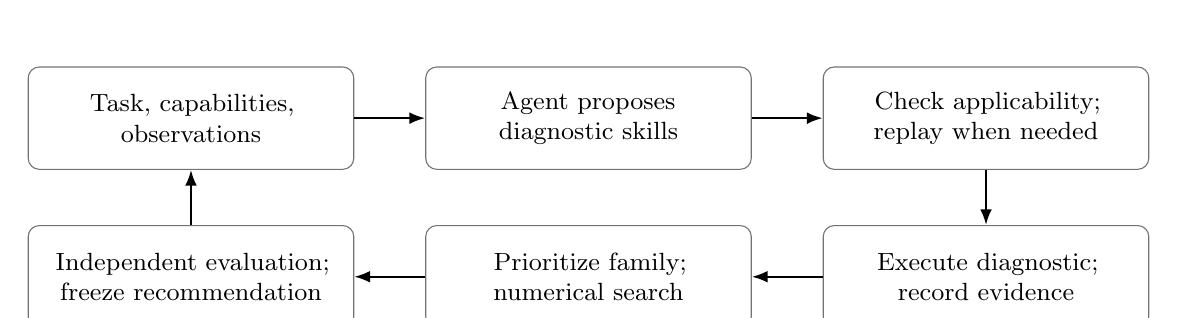
\begin{tikzpicture}[node distance=7mm and 9mm,box/.style={draw=black!55,rounded corners,align=center,font=\small,text width=39mm,minimum height=13mm},arr/.style={-{Latex[length=2mm]},thick}]
\node[box] (state) {Task, capabilities,\\observations};
\node[box,right=of state] (agent) {Agent proposes\\diagnostic skills};
\node[box,right=of agent] (gate) {Check applicability;\\replay when needed};
\node[box,below=of gate] (probe) {Execute diagnostic;\\record evidence};
\node[box,left=of probe] (search) {Prioritize family;\\numerical search};
\node[box,left=of search] (eval) {Independent evaluation;\\freeze recommendation};
\draw[arr] (state)--(agent); \draw[arr] (agent)--(gate);
\draw[arr] (gate)--(probe); \draw[arr] (probe)--(search);
\draw[arr] (search)--(eval); \draw[arr] (eval)--(state);
\end{tikzpicture}
\caption{Proposed control loop. The diagram specifies a design, not a completed implementation. Updates to skill evidence retain raw run provenance.}
\label{fig:architecture}
\end{figure}

\section{Integration Plan and Algorithm}
\subsection{SGLang and P800 adapter boundary}
The adapter will expose capability discovery, deployment, observation collection, diagnostic execution, benchmark execution, restoration, and configuration freezing. Logical parameters are translated to flags only after checking the deployed version. The controller operates outside the token-generation hot path. It is not proposed as a per-token scheduler.

The capability manifest records model and tokenizer identifiers, weight and KV types, runtime and plugin revisions, attention implementation, parallel configurations, graph and cache modes, transfer backend, and supported routing. CPU, XPU, PCIe, and NIC topology are inventoried instead of inferred from socket count. Unknown single-card memory, NIC speed, and transport behavior remain unset until measurement. Published plugin support cannot replace acceptance checks on the local image.

Deployment operations carry a resource reservation and restoration plan. Diagnostic probes run on designated experimental resources, and all benchmark parsing and objective computation occur outside agent-editable decisions. The agent can select registered operations, but cannot modify evaluation inputs, metric formulas, or baseline configurations during a comparison. This is an experimental control rather than a separate security contribution.

\subsection{Proposed algorithm}
\begin{quote}\small\ttfamily
Input: task, legal resources, capability manifest, initial skills, budgets.\\
1. Measure a declared initial configuration; create evidence records.\\
2. While budget remains:\\
\hspace*{1em}a. Retrieve compatible skill candidates and context records.\\
\hspace*{1em}b. Request structured diagnostic proposals from the controller.\\
\hspace*{1em}c. Check proposals; read or replay diagnostics as needed.\\
\hspace*{1em}d. Record support, contradiction, or inconclusive evidence.\\
\hspace*{1em}e. Propose a legal configuration with guided/global search.\\
\hspace*{1em}f. Deploy, warm, measure, restore when required; charge all costs.\\
\hspace*{1em}g. Update the optimizer and context-specific skill records.\\
\hspace*{1em}h. Check the declared stop or return-to-diagnosis rule.\\
3. Freeze and independently validate the best measured feasible candidate.\\
Output: configuration and evidence, or no measured feasible configuration.
\end{quote}
This pseudocode defines the intended sequencing. The numerical optimizer, context thresholds, probe costs, and stopping settings must be supplied with the implementation. No runnable implementation is claimed in this draft.

\section{Planned Evaluation}
\subsection{Research questions}
RQ1 asks whether the method reaches a prespecified feasible target faster than constrained numerical search and an ordinary tool-using agent. RQ2 asks whether diagnostic selection changes useful configuration decisions relative to a fixed-rule controller with identical skills. RQ3 asks whether local replay and applicability checks improve skill transfer to held-out contexts. RQ4 asks how the final recommendations compare in resource use and attained service capacity across deployment scales.

\subsection{Testbed, tasks, and splits}
The reported starting testbed is four servers, each with eight P800 cards and dual-socket AMD EPYC 9K84 CPUs; the author reports a 96-core CPU specification and RDMA support. The per-socket interpretation, NUMA presentation, usable device memory, NIC count and rate, driver stack, and software revisions will be recorded from the actual machines. More resources are available in principle, but no specific larger experiment has yet been allocated or measured.

We plan to select two stable model configurations that the deployed backend already supports. Resource points will follow complete-replica feasibility. For illustration, an eight-card replica allows 1P1D on 16 cards and 1P2D on 24 cards; this is an allocation example, not a supported-model claim. Additional points, potentially 32, 48, and 64 cards, will be chosen after preliminary capacity measurement. A model that cannot execute a small PD layout will be marked infeasible at that point rather than replaced within the comparison.

Tasks will include short-input/short-output, long-input/short-output, short-input/long-output, and mixed-length request processes. Open-loop arrivals will be used for service-capacity studies, with fixed-concurrency tests as secondary diagnostics. Source tasks build the skill evidence. Context thresholds and the initial library are then frozen before held-out model, load, or scale tasks. Cold-start, warm-start, and optional within-task updates are reported separately.

\subsection{Baselines and component attribution}
\begin{table}[t]
\centering\small
\begin{tabularx}{\linewidth}{@{}>{\raggedright\arraybackslash}p{36mm}YY@{}}
\toprule
Method & Shared conditions & Purpose \\
\midrule
Tuned native serving & Colocated/chunked-prefill and native PD; fixed model and precision & End-to-end engineering reference \\
Constrained optimizer & Same legal space, budgets, and measurement protocol & Benefit beyond numerical search \\
Fixed-rule controller & Same skills, observations, and initial knowledge & Necessity of LLM decisions \\
Tool-using agent & Same model and tools; ordinary feedback and log retrieval & Benefit beyond generic agent orchestration \\
Unconditional skill reuse & Same library; no local applicability/replay mechanism & Cost of incorrect transfer \\
Complete proposal & All declared components & Combined effect and overhead \\
\bottomrule
\end{tabularx}
\caption{Planned comparisons. Adapting ideas from prior systems must be identified as an adaptation, not as running the original implementation.}
\end{table}

A source-aware or rule-accumulating agent inspired by STELLAR or SysInsight is an important strong baseline. If their original implementations cannot control SGLang, an adaptation will be described precisely and supplied with the same evidence and tools. We will not reuse reported speedups from unrelated hardware as quantitative baselines. Ablations will remove active diagnosis, replace skill records with raw-log retrieval, disable applicability replay, and remove global exploration, one mechanism at a time.

\subsection{Metrics, uncertainty, and resource accounting}
Primary metrics are allocation-time and elapsed time to a prespecified target, joint SLO attainment, and final measured resource use at the same offered workload. Secondary metrics include output-token throughput, actual input/output lengths, per-request TTFT/TPOT, token-level inter-token latency, failed configurations, redeployments, and diagnostic actions. P99 results require adequate sample sizes and explicit uncertainty. Diagnostic precision will be reported only for cases with controlled or independently established explanations.

We plan at least three independent repeats of core serving points and multiple controller/search seeds, initially five where affordable. Run order will be randomized or interleaved. Paired comparisons will use the same workload realizations. Requests within one overloaded run are not treated as independent repetitions of the entire tuning process. Unreached targets will be reported as censored outcomes, not dropped when calculating time-to-target.

Thresholds, model selection, search ranges, stopping conditions, the agent prompt, generation settings, and token budgets will be fixed before final evaluation. Agent inference will use separate capacity or have its interference explicitly measured. Parallel searches will share an equal resource ceiling or be compared using an equal allocation-time budget. Offline library construction and online tuning costs will be separated, with amortization reported rather than assumed.

\subsection{Mechanism tests and decision consequences}
The first mechanism test compares isolated transfer, isolated decode, and their controlled concurrent execution when the backend exposes suitable operations. Another compares a stage-capacity recommendation with end-to-end configuration ranking. These tests establish whether the hypothesized ambiguity exists on this platform; they do not automatically establish a novel system mechanism.

For each successful diagnostic, we will trace the decision chain: observations, alternatives considered, chosen probe, probe outcome, changed search priority, selected configuration, and independent validation. For an incorrect diagnostic, we will report the wasted cost and whether replay or global exploration recovered. This analysis connects the skill mechanism to a measurable outcome rather than treating explanation quality as a proxy for performance.

\section{Results: Evidence to Be Added}
\status{No measurements have been obtained for this manuscript. This section defines the evidence required to complete the paper. It must not be rewritten as a results claim until run records and analyses exist.}
The main results will address RQ1--RQ4 with paired uncertainty estimates. Required figures are: time-to-target and attained-quality-over-budget curves; resource--service-capacity frontiers; diagnostic outcomes and their decision consequences; held-out skill transfer with and without replay; and overhead/failed-action breakdowns. No synthetic speedup plot is included.

\begin{table}[h]
\centering\small
\begin{tabularx}{\linewidth}{@{}>{\raggedright\arraybackslash}p{24mm}YY@{}}
\toprule
Evidence & Required analysis & Current status \\
\midrule
E1: mechanism & Competing explanations and controlled diagnostic outcomes & Not measured \\
E2: tuning & Same-budget baselines and time-to-target & Not measured \\
E3: transfer & Frozen source library on held-out contexts & Not measured \\
E4: capacity & Same-load resource use and equal-resource service ability & Not measured \\
E5: ablation & Rules, ordinary agent, replay, and exploration controls & Not measured \\
\bottomrule
\end{tabularx}
\caption{Evidence completion ledger. These entries are status labels, not experimental data.}
\end{table}

Negative findings must change the manuscript's claim. If rules match the LLM controller, we cannot attribute a performance advantage to agent reasoning. If replay costs more than it saves, reuse requires a narrower applicability argument. If no meaningful stage ambiguity appears, the proposed diagnostic design needs revision. A gain over defaults alone will not establish a method contribution.

\section{Limitations and Threats to Validity}
The most immediate limitation is the absence of an integrated implementation and empirical validation. The claimed distinction from agentic storage and database tuners is a research hypothesis. Conditions and conflict handling already exist in prior systems, so the experiment/action representation must deliver observable value beyond renaming contextual rules as skills.

A single accelerator backend limits hardware generalization. Larger resource counts extend scale coverage but do not establish portability to a different accelerator family. Limited observability may prevent reliable diagnosis, while diagnostic instrumentation can perturb execution. Context signatures and thresholds may overfit source tasks. Dynamic co-tenancy, request-length uncertainty, cache state, and network variation may confound intervention outcomes even when only one configuration field is edited.

An LLM controller can omit important alternatives, fabricate parameter semantics, or select expensive probes. Registered actions, evidence references, and independent checking constrain these behaviors but do not prove their absence. Improved tuning time also does not imply better steady-state capacity. Conversely, a more efficient final deployment may require greater tuning cost; both must be reported.

The initial scope excludes automatic kernel rewriting, model-quality tradeoffs, cross-vendor KV interoperability, and production online migration. Public models and reproducible workload descriptions will be preferred; disclosure of actual code, machine details, and traces depends on the organization's permitted publication scope. Unavailable artifacts will be listed explicitly rather than described as released.

\section{Conclusion}
This manuscript proposes a diagnostic-skill abstraction and controller design for configuring PD-disaggregated LLM serving in SGLang. The central hypothesis is that explicitly selecting diagnostic experiments and revalidating their reuse conditions can improve decisions about coupled stages and variable resource allocations. The draft defines a concrete method and an evaluation capable of rejecting that hypothesis. Implementation, evidence collection, and quantitative conclusions remain future work for this manuscript.

\appendix
\section{Implementation Decisions That Must Be Frozen}
Before final experiments, the artifact must specify: the model and precision identifiers; SGLang, plugin, and transport revisions; the mapping from logical actions to supported operations; controller model and prompts; search algorithm and settings; skill contexts and replay thresholds; cost-accounting protocol; arrival and drain semantics; SLOs and timeouts; source/validation/test splits; random seeds; and the conditions for stopping. These are open implementation decisions, not omitted experimental findings.

\section{Claim-to-Evidence Map}
\begin{tabularx}{\linewidth}{@{}YY@{}}
\toprule
Candidate claim & Minimum supporting evidence \\
\midrule
Diagnostic selection improves tuning decisions & Same-tool rule and agent controls; decisions linked to held-out performance \\
Applicability replay reduces negative transfer & Frozen source library; changed-context tasks; unconditional-reuse and cost ablations \\
Resource recommendations are efficient & Same workload/SLO; measured feasible resource comparison; stability and uncertainty \\
The method is practical on P800 & Versioned integrated artifact; acceptance checks; complete overhead and failure records \\
\bottomrule
\end{tabularx}

{\small
\setlength{\bibsep}{5pt plus 1pt minus 1pt}
\bibliographystyle{plainnat}
\bibliography{references}
}
\end{document}
